% Ce document et sa source sont disponibles à l'adresse
% https://github.com/dmegy/L3/tree/main/beamerMagistere
% lien de téléchargement direct du pdf :
% https://raw.githubusercontent.com/dmegy/L3/main/beamerMagistere/beamerMagistere.pdf

\documentclass[slidetop,11pt]{beamer}
\graphicspath{{Images/}}
\usepackage[T1]{fontenc}
\usepackage{graphicx}
\usepackage{multimedia}
\usepackage[utf8]{inputenc}
\usepackage[frenchb]{babel}
\usepackage{url,qrcode}
\usepackage{hyperref}


\def\R{\mathbb{R}}
\def\Z{\mathbb{Z}}
\def\bS{\mathbb{S}}
\def\cC{\mathcal{C}}
\def\HH{\mathbb{H}}
\def\cH{\mathcal{H}}
\def\bd{\partial}


\usetheme{JuanLesPins}
\usecolortheme{seahorse}

\title{Magistère de Mathématiques Poincaré\\ Présentation de la formation}
\author{D. Mégy}
%\institute{Institut élie Cartan de Lorraine, UMR 7752}
%\logo{
\includegraphics[height=1cm]{Logo-MMP-noir-2}}


\begin{document}


  
%\begin{frame}
%\titlepage
%\end{frame}

\begin{frame}
\begin{center}

\includegraphics[height=7cm]{images/Logo-MMP-noir-cropped}
\end{center}
\end{frame}  

\begin{frame}
\frametitle{Table des matières}
\tableofcontents
\end{frame}

\section{Présentation générale de la formation et admission}

\begin{frame}
\begin{center}

\includegraphics[height=1.5cm]{images/Logo-MMP-noir-2}
\end{center}
Le \textbf{Magistère de Mathématiques Poincaré} est une formation sélective de haut niveau de \textbf{3 ans} proposée à \textbf{Nancy} et accessible sur dossier après une deuxième année de licence de mathématiques (L2) ou deux années de classes préparatoires, englobant le cursus L3, M1, M2 classique.
\bigskip

En plus des diplômes nationaux de la \textbf{Licence} et du \textbf{Master}, la formation est sanctionnée par un \textbf{diplôme universitaire de Magistère}, délivré lors de l'obtention du Master.
\end{frame}

\begin{frame}
Le Magistère de Mathématiques Poincaré s'appuie sur l'environnement scientifique de la recherche faite à l'Institut Elie Cartan de Lorraine (IECL) et propose une palette d'activités enrichissant le cursus classique licence/master prévoyant entre autres :
\begin{itemize}
\item 5 enseignements supplémentaires sous la forme de cours classiques.
\item Un mémoire d'initiation à la recherche au niveau L3.
\item Un stage d'application des mathématiques en M1.
\item Deux « Masterclasses » une en M1, une en M2.
\item Un séminaire du Magistère mensuel d'initiation à la recherche.
\item Des séances de problèmes d'écrits de concours.
\end{itemize}

\end{frame}

\begin{frame}
\frametitle{Procédure d'admission}

\textbf{Admission en première année}

\bigskip
Dépôt de candidature sur le site eCandidat de l'université de Lorraine : \og DU Magistère de Mathématiques Poincaré\fg : \\
\url{https://ecandidat.univ-lorraine.fr}

\bigskip
\textbf{Admission directe en deuxième année}

\bigskip
- Dépôt de candidature au Master de mathématiques, parcours MFA sur le site MonMaster.\\
- Dans un second temps, si la candidature en Master est acceptée, candidature au DU Magistère \url{https://ecandidat.univ-lorraine.fr}


\end{frame}



\section{Première année de Magistère}
% =========================

\subsection{Cours du cursus standard de Licence (L3)}
% ------------------------------------

\begin{frame}
\frametitle{Magistère 1A : cours communs de Licence S5}
\begin{itemize}
\item \textbf{Algèbre 3} (6 ECTS) : théorie des groupes jusqu'aux théorèmes de Sylow
\item \textbf{Intégration et probabilités} (9 ECTS) : théorie de la mesure, intégrale de Lebesgue, variables aléatoires mesurables
\item \textbf{Topologie et analyse hilbertienne} (6 ECTS) : Topologie, espaces fonctionnels, espaces de Hilbert
\item Une option (6 ECTS) parmi \textbf{Calcul formel} (arithmétique, cryptographie, corps finis) et \textbf{Analyse numérique} (analyse numérique matricielle, LU, QR...)
\item \textbf{Anglais}, et \textbf{Mathématiques en anglais} (3 ECTS)
\end{itemize}
\end{frame}


\begin{frame}
\frametitle{Magistère 1A : cours communs de Licence S6}


\begin{itemize}
\item \textbf{Algèbre 4} (6 ECTS) : anneaux, corps, polynômes symétriques, arithmétique
\item \textbf{Analyse complexe} (6 ECTS) : fonctions holomorphes, théorie de Cauchy, résidus, Rouché
\item \textbf{Calcul différentiel} (6 ECTS) : calcul différentiel dans un Banach : inversion locale, EDO, Cauchy-Lipschitz
\item \textbf{Probabilités et statistique} (9 ECTS) : convergence des v.a., transformée de Fourier, théorème central limite, estimateurs.
\item \textbf{TIPE/Stage} (3 ECTS) : stage d'initiation à la recherche en mathématiques en laboratoire, mémoire et soutenance
\item \textbf{Anglais} et \textbf{Mathématiques en anglais} (3 ECTS)
\end{itemize}
\end{frame}


\subsection{Cours supplémentaires de Magistère 1A}
% ------------------------------------
\begin{frame}
\frametitle{Magistère 1A : cours supplémentaires (automne)}

\textbf{Analyse harmonique et applications en théorie des nombres} (6 ECTS, 30hCM+30hTD)

Ce cours comportera deux parties, l'une de présentation de l'analyse de Fourier et l'autre d'application à la théorie analytique des nombres, dont une preuve du célèbre théorème des nombres premiers.
\begin{center}
\includegraphics[scale=.2]{images/fourier2.jpg} 
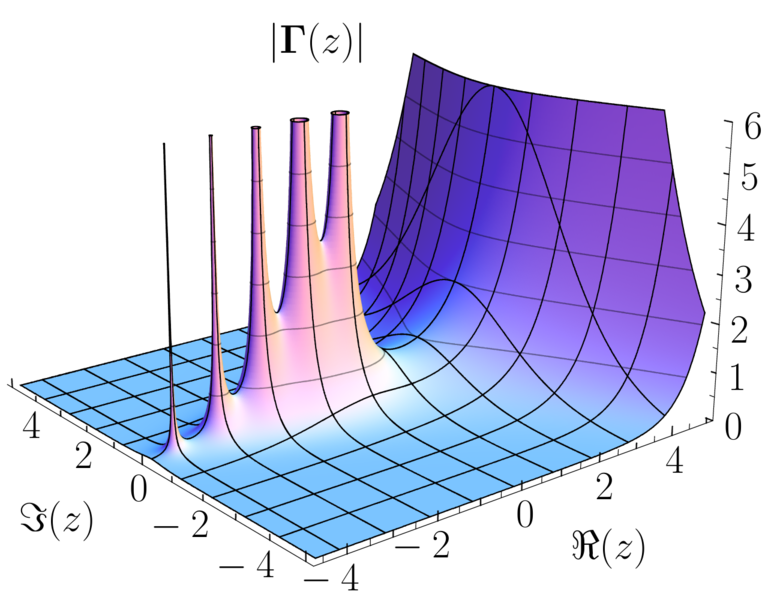
\includegraphics[scale=.2]{images/Gamma_abs_3D.png}
% image wikipedia https://en.m.wikipedia.org/wiki/File:Gamma_abs_3D.png
% trouver une image mieux adaptée, plus analyse harmonique qu'analyse complexe
\end{center}

\end{frame}

\begin{frame}
\frametitle{Magistère 1A : cours supplémentaires (printemps)}

\textbf{Mécanique quantique} (3 ECTS, 14h CM+16h TD)

Cours mutualisé avec la licence de physique théorique.
L'objectif de ce cours est d'introduire la théorie de la mécanique quantique (relation d'incertitudes, processus de mesures) et ses implications. 
\begin{center}
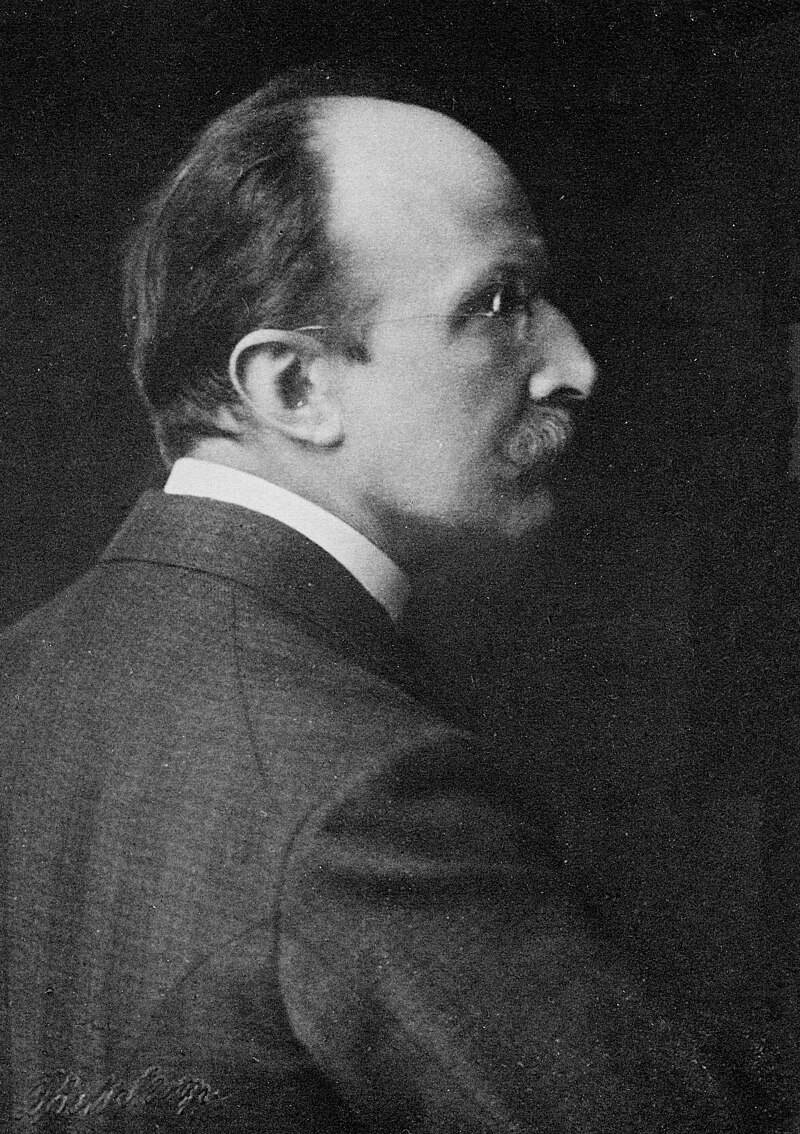
\includegraphics[height=4.3cm]{Max_Planck_Nobel_1918.jpg}$\quad$
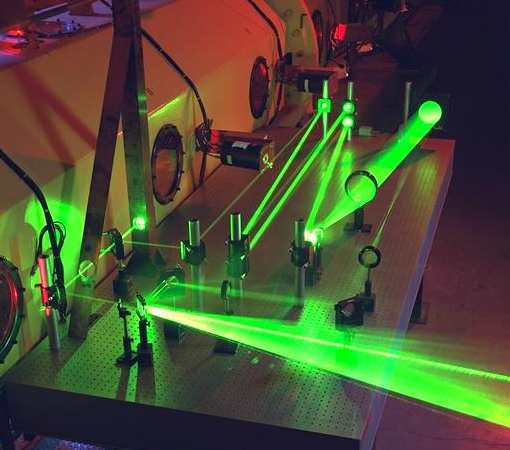
\includegraphics[height=4.3cm]{Laser_optique.jpg}
% source : wikipedia page mecanique quantiqe et max Planck
\end{center}
\end{frame}

\begin{frame}
\frametitle{Magistère 1A : cours supplémentaires (printemps)}

\textbf{Équations différentielles : géométrie, dynamique et chaos}\\
(3 ECTS, 16hCM+14h TD)

Dans ce cours, nous explorerons les bases des systèmes dynamiques, aussi appelées \og théorie du chaos\fg, avec pour fil conducteur un célèbre article du physicien Lorenz qui introduisit la notion d'effet papillon.
\begin{columns}[c]
\begin{column}{6cm}
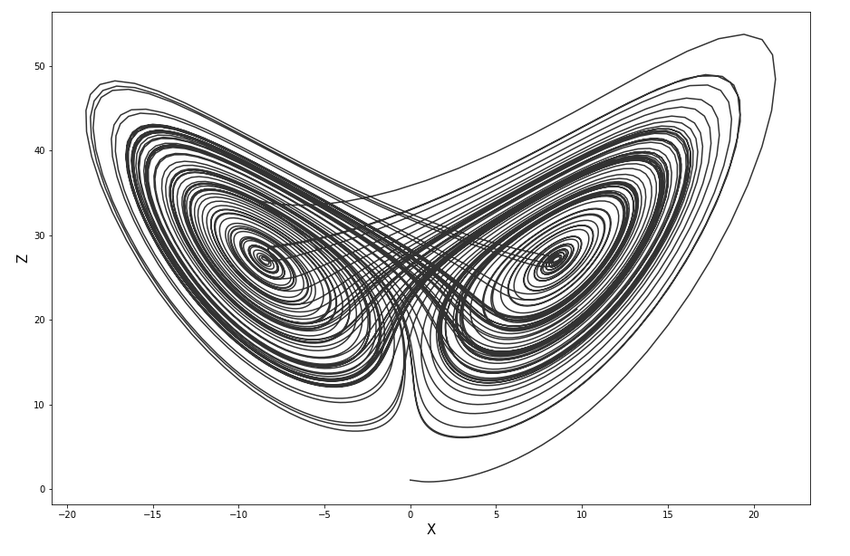
\includegraphics[scale=.2]{images/Lorenz-Attractor-in-2D-space.png}
% crédits : Anton Koshelev DOI:10.48550/arXiv.2104.14190
% image en CCBY NC, rajouter la référence
% trouver une meilleure image...
\end{column}
\begin{column}{5cm}
Vidéo d'introduction: \\
\url{www.chaos-math.org}\\
\qrcode{https://www.chaos-math.org/fr.html}
\end{column}
\end{columns}


\end{frame}

\subsection{Activités supplémentaires de Magistère 1A}
% ------------------------------------
\begin{frame}
\frametitle{Magistère 1A : activités supplémentaires de Magistère}

\begin{itemize}
\item \textbf{Stage d'initiation à la recherche}. Ce stage remplace le TIPE de L3 et le stage obligatoire de licence. Il est encadré par les enseignants-chercheurs de l'IECL et donne lieu à un mémoire et à une soutenance.
\item \textbf{Séminaire du Magistère} : Le séminaire est un endroit où les magistériens peuvent rencontrer les chercheurs.
En particulier, des collègues mathématiciens viennent pour exposer les problèmes qui les intéressent et introduire des objets mathématiques au cœur de leurs recherches.
\end{itemize}
\end{frame}

\subsection{Préparation aux concours en fin de L3/1A}
% ------------------------------------

\begin{frame}
\frametitle{Préparation aux concours bac+3}

Certaines grandes écoles recrutent à l’issue d’une Licence, à bac+3.
C’est le cas de l’École Polytechnique (intégration en première année), ou des Écoles Normales Supérieures de Lyon, de Rennes ou Paris-Saclay (intégration en première ou deuxième année avec statut complet d’élève normalien$\cdot$ne) et de quelques autres (CentraleSupélec). 

\bigskip
Le magistère encourage  les étudiants intéressés à présenter ces concours et propose des séances d’écrits de préparation et du matériel pédagogique en appui.
%La préparation aux écrits de concours bac+3 permet également de commencer à se préparer aux écrits d'agrégation qui ont lieu deux ans plus tard.

\bigskip
Les étudiants qui réussissent ces concours quittent le magistère dès la fin de la première année.
\end{frame}

\begin{frame}
\frametitle{Plus d'informations sur les concours}


\begin{itemize}
\item \og Second concours\fg{} de l'ENS Lyon : intégration en première année avec statut d'élève. \url{https://www.ens-lyon.fr/formation/admission/procedures-dadmission/second-concours}
\item \og Concours deuxième année\fg{} des ENS Rennes et Saclay :  intégration en deuxième année avec statut d'élève. \url{https://www.ens-rennes.fr/admission/concours2a/mathematiques}
\item École Polytechnique : intégration avec statut de polytechnicien$\cdot$ne en première année. \url{https://www.polytechnique.edu/admission-cycle-ingenieur/candidats-francais-filiere-universitaire}
% notice pdf : https://www.polytechnique.edu/admission-cycle-ingenieur/sites/admission/files/content/2025%20FUF%20NOTICE%20CANDIDATS.pdf
\item Concours universitaire du Groupe Centrale: \url{https://www.groupe-centrale.com/concours-universitaire/}
\end{itemize}

\end{frame}


\section{Deuxième année de Magistère}
% =========================

\subsection{Cours communs de Master1}
% ------------------------------------
\begin{frame}
\frametitle{Magistère 2A : cours communs de Master (automne)}
\begin{itemize}
\item Algèbre et géométrie (6 ECTS)
\item Analyse (7 ECTS)
\item Calcul différentiel/EDO - calcul matriciel (2 modules, 7 ECTS)
\item Statistiques et probabilités (7 ECTS)
\item \textbf{Anglais} (3 ECTS)
\end{itemize}

\bigskip
Programme détaillé des UE: 
\url{https://iecl.univ-lorraine.fr/wp-content/uploads/2024/10/s7-programmes.pdf}
\end{frame}


\begin{frame}
\frametitle{Magistère 2A : cours communs de Master (printemps)}
\begin{itemize}
\item Algèbre et arithmétique (6 ECTS)
\item Analyse fonctionnelle (6 ECTS)
\item Géométrie (6 ECTS)
\item Probabilités (6 ECTS)
\item TER (3 ECTS)
\item \textbf{Mathématiques en anglais} (3 ECTS)
\end{itemize}


\bigskip
Programme détaillé des UE: 
\url{https://iecl.univ-lorraine.fr/wp-content/uploads/2024/10/s7-programmes.pdf}
\end{frame}

\subsection{Cours supplémentaires de Magistère 2A}
% ----------------------------------

\begin{frame}
\frametitle{Magistère 2A : cours supplémentaires de Magistère}

\textbf{Logique et modèle de calcul }
(S7, 22h CM+ 22h TD, 4 ECTS)

L'objectif de ce cours est de présenter à la fois la logique comme modèle de calcul et outil de programmation et d'aborder la notion de calculabilité et les différents modèles de calcul. 

Cours mutualisé avec le Master d'informatique théorique de Nancy.

\end{frame}


\begin{frame}
\frametitle{Magistère 2A : cours supplémentaires de Magistère}

\textbf{Analysis Situs (Topologie algébrique)}
(S8, 30h de CM + 30h de TD, 6 ECTS)

\bigskip
L'objectif de ce cours est l'introduction à la topologie algébrique (originalement appelée \textit{Analysis Situs} par Poincaré) des variétés telle qu'elle a été conçue par Henri Poincaré dans une série de six mémoires révolutionnaires.

Le cours s'appuiera entre autres sur le magnifique travail effectué par les auteurs du site  \url{http://analysis-situs.math.cnrs.fr}.


\end{frame}

\subsection{Activités supplémentaires de Magistère 2A}
%------------------------------------

\begin{frame}
\frametitle{Magistère 2A : Stage d’application des mathématiques}

L’objectif du stage de deuxième année de Magistère est de familiariser les étudiants avec les applications des mathématiques dans d’autres domaines. Le stage dure environ 4 semaines est il est en général effectué dans la période entre la fin du M1 et la rentrée du M2.

Le stage peut être effectué dans une unité de recherche universitaire (en dehors des mathématiques) ou dans une entreprise ou une administration.
\end{frame}


\begin{frame}
\frametitle{Magistère 2A : Première Masterclass}

Les Masterclasses sont des mini-conférences d'une semaine destinées aux  étudiants.

La Masterclass en  M1 propose des cours sur les thèmes qui feront l'objet du Master 2 MFA de l'année suivante.

Dernières éditions :
\begin{itemize}
\item 2025 : Géométrie Riemannienne \& Equations aux Dérivées Partielles,  \url{https://iecl.univ-lorraine.fr/masterclassm12025/}
\item 2024 : Groupes de Lie et probabilités \url{https://dev-iecl.univ-lorraine.fr/masterclassm12024/}
\end{itemize}

%La Masterclass en fin de M2 constitue le point d’orgue de l’année. Des mini-cours et des exposés avancés introduisent les étudiants à des directions de recherche actuelles. Dernières éditions :  groupes de Lie et probabilités (2024) , géométrie riemannienne et EDP (2025). 
\end{frame}

\section{Troisième année de Magistère}
% =========================
\begin{frame}
\frametitle{Troisième année de Magistère}

La troisième année de magistère est entièrement dédiée à l'obtention d'un \textbf{Master 2 Recherche (M2R)}.

Le Magistère offre une seconde Masterclass de fin de M2R qui fait la jonction entre les cours de Master et les travaux de recherche actuelle dans les domaines en question. Les étudiants bénéficient toujours de l'organisation du séminaire du magistère.

\bigskip
Les étudiants ont l'opportunité, après approbation des responsables du magistère, d'effectuer ce M2R dans une \textbf{autre université} que l'université de Lorraine.

\bigskip
Les étudiants peuvent également demander une année de césure entre la deuxième et la troisième année de magistère pour préparer le concours de l'\textbf{agrégation de mathématiques}.

\end{frame}


\begin{frame}
\frametitle{Questions ?}

\begin{center}
{\LARGE \bf Merci pour votre attention !!}

\bigskip
\qrcode[hyperlink, height=4cm]{https://iecl.univ-lorraine.fr/magistere-poincare}

\bigskip
\url{https://iecl.univ-lorraine.fr/magistere-poincare}

\bigskip
Ce document est disponible à l'adresse\\
\url{https://raw.githubusercontent.com/dmegy/L3/main/beamerMagistere/beamerMagistere.pdf}
\end{center}
\end{frame}
  \end{document}
  